% =====================================================================
%  IEEE Project Report -- Two-Way Set-Associative Cache with LRU
%  Template : IEEEtran (conference mode)
%  Build    : tectonic IEEE_Cache_Project_Report.tex
%         or: pdflatex IEEE_Cache_Project_Report.tex (run twice)
%
%  Section map required by the course guidelines
%    Phase I : Abstract, Literature Review, Proposed Solution,
%              Individual Contributions, References
%    Phase II: + Results and Discussion, Conclusion
% =====================================================================
\documentclass[conference]{IEEEtran}

\usepackage[utf8]{inputenc}
\usepackage{amsmath}
\usepackage{newtxtext,newtxmath}   % Times, as used by IEEE publications
\usepackage{graphicx}
\usepackage{booktabs}
\usepackage{array}
\usepackage{url}
\usepackage{tikz}
\usetikzlibrary{arrows.meta,positioning,shapes.misc}
\usepackage{pgfplots}
\pgfplotsset{compat=1.17}

\renewcommand{\arraystretch}{1.15}

\begin{document}

\title{Design and Evaluation of a Two-Way\\Set-Associative Cache with LRU Replacement}

\author{
\IEEEauthorblockN{Meghna Nair, Pranjal Shukla, Shreya Narayani, Ritesh Kumar, Nikith Gowda B S}
\IEEEauthorblockA{Final Project Report \textbar{} November 2026}
}

\maketitle

% ---------------------------------------------------------------------
\begin{abstract}
This report presents a modular Verilog implementation of a two-way
set-associative cache with least recently used (LRU) replacement. The
design stores four one-byte cache lines in two sets and uses a four-bit
address, parallel tag comparison, valid-bit qualification, and one
replacement bit per set. A six-state controller accepts a read request,
performs lookup, fetches missing data, and returns one response. The
repository was evaluated using Icarus Verilog. Its integration test
reported 53 successful checks and no failures. Additional directed traces
were run against the unmodified cache RTL and compared with an
equal-capacity direct-mapped software model. For an alternating
two-address conflict trace, the two-way cache achieved an 87.50\% hit
rate, compared with 0\% for the direct-mapped model. A three-address
same-set loop exposed the opposite trade-off: two-way LRU produced no
hits while direct mapping achieved 27.78\%. These results demonstrate
correct replacement behavior and show that the benefit of associativity
depends on the access pattern. Resource discussion is based on logical
storage and datapath structure; FPGA utilization and post-route timing
have not been measured.
\end{abstract}

\begin{IEEEkeywords}
Cache memory, set associativity, LRU replacement, Verilog, finite-state
machine, memory hierarchy.
\end{IEEEkeywords}

% =====================================================================
\section{Introduction}

The project objective is to implement a two-way cache, verify its
selection and replacement behavior, and compare it with a direct-mapped
cache. The implementation~\cite{repo} is deliberately small: sixteen
backing-memory locations and four cache entries make every mapping
decision observable. This scale is appropriate for learning RTL
organization, checking waveforms, and constructing traces whose expected
outcomes can be calculated by hand.

A cache hit is useful only if it returns the correct data for the
accepted request. Consequently, the design must coordinate address
capture, tag lookup, replacement, memory timing, and response
generation. Merely obtaining a high hit rate does not establish
functional correctness. A stale address, an invalid matching tag, or an
incorrectly updated replacement bit can produce apparently plausible
statistics while returning the wrong byte.

\subsection{Motivation and Project Scope}

Direct mapping assigns each block to one cache entry. Two-way
organization provides two possible entries within the selected set.
This flexibility can retain two addresses that would repeatedly
overwrite one another in a direct-mapped cache. It requires an
additional comparison path, a way-selection multiplexer, and
replacement state. The project therefore examines a concrete trade-off
between placement flexibility and hardware structure rather than
treating associativity as a universal improvement.

The implemented top-level interface supports reads only. Each miss
allocates one byte, and no block offset is required. There are no CPU
write inputs, dirty bits, write-back transactions, prefetching,
coherence messages, or multiple outstanding requests. The
backing-memory module has write ports, but the top level disables them.
These boundaries are important when interpreting both verification
results and possible FPGA use.

\subsection{Evidence and Evaluation Boundary}

The source snapshot is Git commit \texttt{c8b1374}, evaluated on
November 16, 2026. It contains eight RTL files and eight testbench
files. The report distinguishes three evidence types: behavior
implemented in those files, results reproduced by simulation during
report preparation, and analytical or proposed extensions. The
supplementary trace experiment does not modify the repository RTL.

The repository does not yet contain a direct-mapped RTL baseline or a
completed synthesis report. Accordingly, the comparison uses a simple
direct-mapped reference model with the same four-byte data capacity.
This supports a controlled hit-rate comparison, but it does not
establish a measured timing or area advantage over a second hardware
implementation.

\subsection{Main Technical Findings}

The implemented lookup correctly gives preference to a hit, then an
invalid way, and finally the LRU victim. Accessing either way makes the
other way the next victim. Simulation confirms that successful reads
return the initialized memory value and that the selected directed
traces have the expected hit and miss counts. The controller also
prevents requests presented while busy from overwriting the active
address.

The remainder of the report reviews relevant cache concepts, describes
the architecture and controller, states the verification methodology,
discusses measured and model-based results separately, and records the
individual contribution of each team member.

% =====================================================================
\section{Literature Review}

\subsection{Placement and Locality}

Cornell's CS~3410 cache notes~\cite{cornell} explain temporal locality
as repeated access to the same data and spatial locality as access to
nearby addresses. They develop direct-mapped and associative placement
as ways to retain useful memory contents. This provides the conceptual
basis for the repeated-address and conflict traces in this report.
Since the implemented line is one byte, fetching a location does not
automatically bring its neighbors into the cache. The design therefore
demonstrates reuse more directly than spatial prefetch benefits.

At equal data capacity, changing associativity also changes the number
of sets. For this project, direct mapping uses four sets, whereas
two-way organization uses two. Thus, the mapping function changes along
with the number of available ways. A fair comparison must hold line
size and total data capacity constant and report the exact address
sequence; otherwise, an improvement may come from extra capacity or a
different workload.

\subsection{Replacement and Identification}

The UC Berkeley CS~61C material~\cite{berkeley} separates placement,
identification, replacement, and write policy. It also explains why
valid bits are needed and why candidate tags can be checked in parallel.
This separation is reflected in the repository's decoder, comparator,
hit/miss selector, cache array, and LRU modules. In particular, tag
equality alone is insufficient: an entry that has not been filled must
not produce a hit.

For two ways, exact LRU needs only one bit per set because there are
only two possible recency orderings. The implementation records the
next victim rather than an access timestamp. If way~0 is accessed,
way~1 becomes the victim; if way~1 is accessed, way~0 becomes the
victim. Updating replacement state on a hit matters because repeated
accesses change which resident line should survive the next miss.

\subsection{Conflict Misses in Prior Research}

Jouppi~\cite{jouppi} studied small associative structures that reduce
mapping conflicts in direct-mapped caches. The paper considers miss
caches, victim caches, and stream buffers. Its relevance here is the
recognition that cache misses can arise from restricted placement even
when the active data set is small. The present implementation uses two
ways inside each set rather than a separate victim cache. The paper's
benchmark results are not treated as measurements of this project.

\subsection{Literature Synthesis and Design Choice}

The reviewed work motivates a compact experiment: keep total capacity
fixed, select traces that distinguish compulsory misses from repeated
conflicts, and observe whether replacement state preserves the recently
used entry. The project's contribution is an educational RTL
realization and reproducible evaluation of these mechanisms. It does
not propose a new replacement algorithm or claim to outperform
production cache designs.

\begin{table}[!t]
\caption{Relation Between Sources and This Project}
\label{tab:sources}
\centering
\begin{tabular}{p{0.21\columnwidth}p{0.3\columnwidth}p{0.33\columnwidth}}
\toprule
Source & Relevant concept & Application \\
\midrule
Cornell~\cite{cornell} & Locality and placement & Repeat and conflict traces \\
UC Berkeley~\cite{berkeley} & Valid bits and replacement & Qualified hits and LRU \\
Jouppi~\cite{jouppi} & Mapping conflicts & Motivation for flexible placement \\
Icarus~\cite{icarus} & Compile and simulate RTL & Reproduced test execution \\
\bottomrule
\end{tabular}
\end{table}

% =====================================================================
\section{Proposed Solution}

\subsection{Cache Organization and Address Format}

The cache contains two sets with two ways per set. Each line stores an
eight-bit data value, a three-bit tag, and one valid bit. The four-bit
CPU address selects one of sixteen one-byte memory locations. Address
bit~0 selects the set, while bits~3 through~1 form the tag. A block
offset is absent because each block contains exactly one addressable
byte.

For an address $A$, the implemented mapping is
$\mathit{set} = A \bmod 2$ and $\mathit{tag} = \lfloor A/2 \rfloor$.
Addresses 0, 2, 4, and 6 therefore share set~0 but have distinct tags.
Addresses 1, 3, 5, and 7 share set~1. Within a set, either way may hold
the requested address. The hardware way number is not part of the CPU
address; the lookup and replacement logic select it.

\begin{table}[!t]
\caption{Implemented Cache Configuration}
\label{tab:config}
\centering
\begin{tabular}{ll}
\toprule
Property & Value \\
\midrule
Address width / data width & 4 bits / 8 bits \\
Sets / ways per set & 2 / 2 \\
Cache lines / line size & 4 / 1 byte \\
Data capacity & 4 bytes \\
Tag / index / offset & 3 / 1 / 0 bits \\
Backing memory & 16 locations $\times$ 8 bits \\
Replacement state & 1 bit per set \\
Access policy & Read-only, allocate on miss \\
\bottomrule
\end{tabular}
\\[4pt]
\parbox{0.95\columnwidth}{\footnotesize These widths are fixed in the
current RTL rather than exposed as generic parameters. Scaling the
design would require consistent changes across the decoder, arrays,
controller, memory interface, and testbench expectations.}
\end{table}

\subsection{Modular Datapath}

The top-level \texttt{cache\_2way} module connects the controller to
the address decoder, cache array, comparators, hit/miss selector, LRU
unit, and backing memory (Fig.~\ref{fig:block}). The decoder receives
the captured request address through \texttt{mem\_address}. This is
intentional: the cache lookup uses the active transaction, not a
changing external CPU address.

\begin{figure}[!t]
\centering
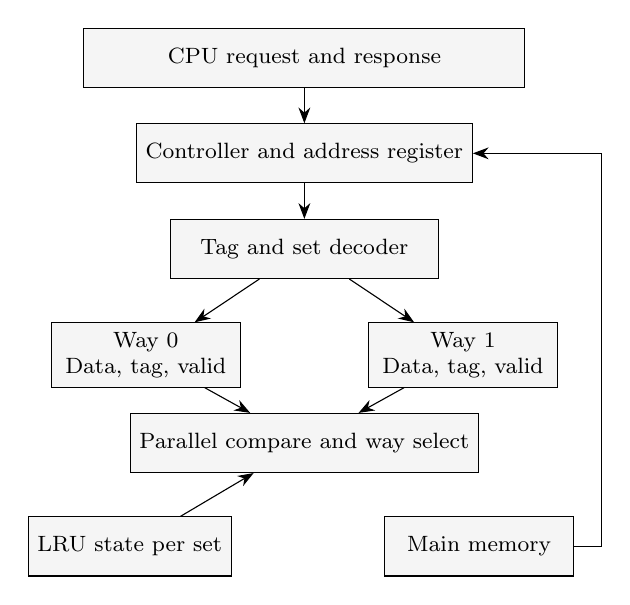
\begin{tikzpicture}[
  blk/.style={draw, fill=gray!8, minimum height=0.75cm, align=center, font=\footnotesize},
  >={Stealth[length=2mm]}, node distance=0.45cm]
  \node[blk, minimum width=5.6cm] (cpu) {CPU request and response};
  \node[blk, minimum width=4.2cm, below=of cpu] (ctrl) {Controller and address register};
  \node[blk, minimum width=3.4cm, below=of ctrl] (dec) {Tag and set decoder};
  \node[blk, minimum width=2.4cm, below left=0.55cm and -0.9cm of dec] (w0) {Way 0\\Data, tag, valid};
  \node[blk, minimum width=2.4cm, below right=0.55cm and -0.9cm of dec] (w1) {Way 1\\Data, tag, valid};
  \node[blk, minimum width=4.2cm, below=1.7cm of dec] (cmp) {Parallel compare and way select};
  \node[blk, minimum width=2.4cm, below=0.55cm of cmp.south west, anchor=north] (lru) {LRU state per set};
  \node[blk, minimum width=2.4cm, below=0.55cm of cmp.south east, anchor=north] (mem) {Main memory};
  \draw[->] (cpu) -- (ctrl);
  \draw[->] (ctrl) -- (dec);
  \draw[->] (dec) -- (w0);
  \draw[->] (dec) -- (w1);
  \draw[->] (w0) -- (cmp);
  \draw[->] (w1) -- (cmp);
  \draw[->] (lru) -- (cmp);
  \draw[->] (mem.east) -- ++(0.35,0) |- (ctrl.east);
\end{tikzpicture}
\caption{Logical organization of the implemented cache. Control and
refill paths are simplified for readability. A signal-level diagram is
provided in \texttt{diagrams/block\_diagram.svg}.}
\label{fig:block}
\end{figure}

The \texttt{cache\_array} module stores four entries using flattened
indices. The expression \texttt{\{set\_index, way\_select\}} identifies
a physical entry. Both ways of the selected set are read
combinationally, while reset and refill writes occur on the rising clock
edge. Clearing valid bits on reset ensures that matching reset tag
values cannot create false hits.

The \texttt{tag\_comparator} module compares the requested tag with the
two stored tags in parallel. The \texttt{hit\_miss\_unit} then
qualifies those matches with the corresponding valid bits. Its
\texttt{selected\_way} output serves two related purposes: it selects
the resident byte on a hit and identifies the refill destination on a
miss. The controller captures this decision before the memory
transaction proceeds.

\subsection{Hit Detection and Way Selection}

Let $V_0$ and $V_1$ denote validity, $T_0$ and $T_1$ the stored tags,
and $T$ the requested tag. The lookup implements
\begin{align}
H_0 &= V_0 \wedge (T_0 = T), \\
H_1 &= V_1 \wedge (T_1 = T), \\
\mathit{Hit} &= H_0 \vee H_1 .
\end{align}

The selection priority is way-0 hit, way-1 hit, invalid way~0, invalid
way~1, and finally the LRU bit (Table~\ref{tab:waysel}). Invalid-way
preference avoids evicting useful data while an empty slot remains.
Way-0 priority also makes the combinational result deterministic if
both comparators match; ordinary operation should not create duplicate
valid copies of the same address in a set.

\begin{table}[!t]
\caption{Way Selection Rules}
\label{tab:waysel}
\centering
\begin{tabular}{lc}
\toprule
Condition in priority order & Selected way \\
\midrule
Valid tag match in way 0 & 0 \\
Otherwise, valid match in way 1 & 1 \\
Otherwise, way 0 invalid & 0 \\
Otherwise, way 1 invalid & 1 \\
Otherwise, both ways occupied & LRU bit \\
\bottomrule
\end{tabular}
\end{table}

\subsection{LRU Update and Refill Behavior}

The \texttt{lru\_unit} contains two one-bit registers, one for each set.
Reset initializes both to zero. When \texttt{update\_en} and
\texttt{access\_valid} are asserted, it writes the complement of
\texttt{access\_way} into the selected set's replacement bit. In the
top level, \texttt{access\_valid} is connected to
\texttt{lru\_update\_en}, so replacement state changes only when the
controller explicitly requests an update.

A hit updates LRU during LOOKUP. A miss updates LRU during FILL after
the memory value has been captured. The newly filled entry is therefore
considered the most recently used. Updating only on misses would be
incorrect: a resident line that is repeatedly read must be protected
relative to the other line, even if neither has been refilled recently.

Consider the sequence 3, 5, 3, 7. All four accesses select set~1. The
first two reads fill different ways. The next read of 3 marks the way
holding 5 as least recently used. The read of 7 then replaces 5 while
retaining 3. This sequence checks the dependency between hit selection
and replacement state; checking returned data alone would not
distinguish a correct victim choice from an unnecessary refill later.

Because the cache is read-only, eviction requires no write-back. There
is no dirty state to inspect, and a miss always requests the addressed
byte from backing memory. A future writable implementation would need
an explicitly selected write policy and additional verification of
memory consistency.

\subsection{Controller and Transaction Sequence}

The \texttt{cache\_controller} implements six states: IDLE, LOOKUP,
MEM\_READ, WAIT\_MEM, FILL, and RESPONSE (Fig.~\ref{fig:fsm}).
\texttt{request\_ready} is asserted only in IDLE. A request is accepted
on a rising edge when \texttt{request\_valid} and
\texttt{request\_ready} are both high; the address is stored in
\texttt{address\_reg}. Only one transaction can be active at a time.

\begin{figure}[!t]
\centering
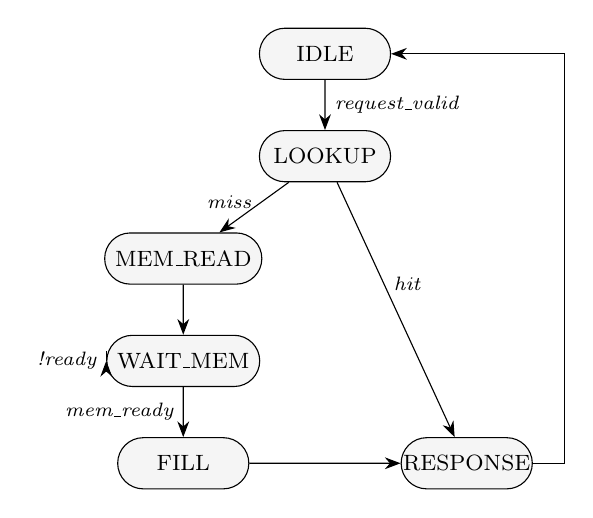
\begin{tikzpicture}[
  st/.style={draw, rounded rectangle, fill=gray!8, minimum width=1.9cm, minimum height=0.65cm, font=\footnotesize},
  lab/.style={font=\scriptsize\itshape},
  >={Stealth[length=2mm]}]
  \node[st] (idle) at (0,0) {IDLE};
  \node[st] (look) at (0,-1.3) {LOOKUP};
  \node[st] (mrd)  at (-1.8,-2.6) {MEM\_READ};
  \node[st] (wait) at (-1.8,-3.9) {WAIT\_MEM};
  \node[st] (fill) at (-1.8,-5.2) {FILL};
  \node[st] (resp) at (1.8,-5.2) {RESPONSE};
  \draw[->] (idle) -- node[right, lab]{request\_valid} (look);
  \draw[->] (look) -- node[left, lab, pos=0.4]{miss} (mrd);
  \draw[->] (look) -- node[right, lab, pos=0.4]{hit} (resp);
  \draw[->] (mrd) -- (wait);
  \draw[->] (wait) -- node[left, lab]{mem\_ready} (fill);
  \draw[->] (fill) -- (resp);
  \draw[->] (resp.east) -- ++(0.4,0) |- (idle.east);
  \draw[->] (wait.west) to[out=200, in=160, looseness=5] node[left, lab]{!ready} (wait.west);
\end{tikzpicture}
\caption{Controller transitions. WAIT\_MEM remains active until
\texttt{mem\_ready}; IDLE waits for a valid request. See also
\texttt{diagrams/controller\_fsm.svg}.}
\label{fig:fsm}
\end{figure}

A hit advances from LOOKUP directly to RESPONSE. The hit byte is
captured into \texttt{response\_data\_reg}, and the accessed way updates
the LRU state. A miss first enters MEM\_READ, which issues one memory
request. WAIT\_MEM captures the returned byte when \texttt{mem\_ready}
is asserted. FILL writes the selected entry and prepares
\texttt{response\_data\_reg}. RESPONSE asserts \texttt{response\_valid}
for one cycle before returning to IDLE.

The top-level \texttt{cache\_hit} signal is qualified by
\texttt{lookup\_active}. It is meaningful during LOOKUP, not at the
later response pulse. A testbench that samples this signal only when
\texttt{response\_valid} is high would incorrectly count hits as misses.
The supplementary experiment counts hit events at the active lookup
clock edge and counts memory reads independently.

There is no \texttt{response\_ready} input. The requester must consume
the response when \texttt{response\_valid} is asserted. This interface
supports request-side backpressure but not response-side backpressure;
connecting it to a system that can stall responses would require an
output holding mechanism.

\subsection{Memory Model and Cycle Accounting}

The \texttt{main\_memory} module contains sixteen eight-bit entries.
Synchronous reset initializes location $A$ to hexadecimal A0 plus $A$,
producing values A0 through AF. A read request returns the selected
value and asserts ready on the next registered update. Simultaneous
read and write requests are rejected in the memory unit, although
writes are disabled in the integrated cache.

\begin{table}[!t]
\caption{Response Timing for the Supplied Memory}
\label{tab:timing}
\centering
\begin{tabular}{clll}
\toprule
Edge & Hit path & Miss path \\
\midrule
0 & Enter LOOKUP & Enter LOOKUP \\
1 & Enter RESPONSE & Enter MEM\_READ \\
2 & Return to IDLE & Enter WAIT\_MEM \\
3 & Available for next request & Enter FILL \\
4 & --- & Enter RESPONSE \\
5 & --- & Return to IDLE \\
\bottomrule
\end{tabular}
\end{table}

Timing in Table~\ref{tab:timing} is measured from the accepting edge to
the assertion of \texttt{response\_valid} after the relevant edge. Under
the supplied memory model, a hit takes one elapsed clock period and a
miss takes four. With the testbench's 10~ns clock period, these
correspond to 10~ns and 40~ns of simulated response latency. They are
not measured FPGA propagation delays or a guarantee of 100~MHz
operation.

Response latency differs from request throughput. The controller spends
a cycle in RESPONSE and does not accept a new request until an IDLE
cycle. Even with \texttt{request\_valid} continuously asserted,
consecutive hits cannot be accepted on every clock. Under this state
sequence, the minimum acceptance spacing is three cycles for hits and
six for misses. Driver-inserted idle time can increase these intervals
further.

% =====================================================================
\section{Verification Methodology}

\subsection{Reproducible Simulation Setup}

The repository was compiled with Icarus Verilog~\cite{icarus} using the
\texttt{-g2012} option and an explicitly selected testbench top. The
RTL source was not edited. Each testbench was compiled separately to
prevent independent stimulus processes from interfering with one
another. The address-decoder bench writes a waveform to
\texttt{simulation/waveforms/address\_decoder.vcd}, so it must be run
from the repository root where that directory exists. Exit status alone
was not used as proof of success: printed checks and failure summaries
were also inspected.

\subsection{Unit and Integration Checks}

Unit tests isolate address decoding, tag comparison, cache storage,
hit/miss selection, LRU state, memory access, and controller
transitions. Integration tests then exercise the complete path from CPU
request to response. The combined approach makes failures easier to
localize: correct replacement-state logic is insufficient if the
controller applies the update to the wrong set or at the wrong time.

\begin{table}[!t]
\caption{Reproduced Repository Test Results}
\label{tab:tests}
\centering
\begin{tabular}{lcc}
\toprule
Testbench & Successful checks & Failures \\
\midrule
\texttt{address\_decoder\_tb} & 16 & 0 \\
\texttt{tag\_comparator\_tb} & 8 & 0 \\
\texttt{cache\_array\_tb} & 9 & 0 \\
\texttt{hit\_miss\_unit\_tb} & 9 & 0 \\
\texttt{lru\_unit\_tb} & 11 & 0 \\
\texttt{main\_memory\_tb} & 5 & 0 \\
\texttt{cache\_controller\_tb} & 20 & 0 \\
\texttt{cache\_2way\_tb} & 53 & 0 \\
\bottomrule
\end{tabular}
\end{table}

The integration bench covers cold misses, repeat hits, filling the
second way, both directions of LRU eviction, independence between sets,
reads across the address range, and request handshaking. It also counts
backing-memory reads to distinguish hits from refills. Its final result
is 53 passed checks and zero failed checks; these are checks, not 53
separate benchmark traces.

\subsection{Additional Trace Experiment}

Eight deterministic traces were evaluated against the original two-way
RTL. Before each trace, the cache and memory were reset and counters
cleared. The driver waited for \texttt{request\_ready}, held each
address through the accepting edge, then awaited
\texttt{response\_valid} with a twenty-cycle timeout. Every returned
byte was compared with hexadecimal A0 plus the requested address.

An independent two-way software model maintained a
least-to-most-recently-used list for each set. On a hit, it moved the
accessed address to the most-recent position. On a miss, it removed the
oldest entry only if the set was full, then inserted the new address.
The RTL's hit count and memory-request count were checked against this
model for every trace. All eight comparisons matched.

This additional test is a reproducible analysis performed for the
report; it checks data, hit totals, and miss totals for the selected
traces and is not exhaustive formal verification of every possible
transaction sequence.

\subsection{Fair Direct-Mapped Baseline}

The direct-mapped model has four one-byte entries, matching the RTL's
four-byte data capacity. Its index is $A \bmod 4$ and its tag is
$\lfloor A/4 \rfloor$, giving two index bits and two tag bits. Each
trace starts with all entries invalid. A hit requires the selected entry
to contain the requested address; a miss replaces that entry immediately
in the functional model.

The baseline has no HDL controller and does not model a clock. It is
used only for hit and miss classification. Both models receive the same
addresses in the same order, use the same line size, and include
compulsory misses. Comparing the two-way cache against a two-entry
direct-mapped cache would confound associativity with capacity and is
intentionally avoided.

\begin{table}[!t]
\caption{Exact Trace Definitions}
\label{tab:traces}
\centering
\begin{tabular}{lp{0.5\columnwidth}c}
\toprule
Trace & Address sequence & $N$ \\
\midrule
Repeat & $[3]\times16$ & 16 \\
Conflict pair & $[0,4]\times8$ & 16 \\
Four-line loop & $[0,1,2,3]\times4$ & 16 \\
One pass & $0,1,\ldots,15$ & 16 \\
Three tags & $[0,2,4]\times6$ & 18 \\
Two sets & $[0,1,4,5]\times4$ & 16 \\
LRU probe & 3, 5, 3, 7, 3, 5, 3, 5 & 8 \\
Mixed & 0, 4, 1, 5, 0, 1, 8, 9, 4, 5, 8, 9, 2, 3, 2, 3 & 16 \\
\bottomrule
\end{tabular}
\end{table}

Addresses in Table~\ref{tab:traces} are decimal; the multiplication
sign means repetition of the entire bracketed sequence. Across the
eight independently reset traces, there are 122 completed accesses.
Resetting between traces prevents the final contents of one test from
biasing the next test's cold-start behavior.

\subsection{Metrics and Interpretation}

For $N$ accepted and completed requests, $H$ hits, and $M$ misses,
$N = H + M$. Hit rate is $100H/N$ percent and miss rate is $100M/N$
percent. In this read-only design, each miss issues one backing-memory
read, so the memory-read count should equal $M$. This equality provides
a useful cross-check on the hit counter.

Average response latency is calculated from observed cycles, not
inferred from hit rate alone. For the supplied memory model, the
expected mean is
\begin{equation}
L = \frac{H + 4M}{N}\ \text{cycles}.
\end{equation}
This equation excludes reset, driver idle cycles, and the extra state
time before the next request can be accepted. A comparison of
end-to-end workload runtime would require a consistent
request-generation policy for both hardware designs.

% =====================================================================
\section{Results and Discussion}

\subsection{Hit-Rate Comparison}

\begin{table}[!t]
\caption{Cold-Start Hit Counts and Hit Rates}
\label{tab:hits}
\centering
\begin{tabular}{lrr}
\toprule
Trace & Direct mapped & Two-way RTL \\
\midrule
Repeat & 15/16 \;93.75\% & 15/16 \;93.75\% \\
Conflict pair & 0/16 \;\phantom{0}0.00\% & 14/16 \;87.50\% \\
Four-line loop & 12/16 \;75.00\% & 12/16 \;75.00\% \\
One pass & 0/16 \;\phantom{0}0.00\% & 0/16 \;\phantom{0}0.00\% \\
Three tags & 5/18 \;27.78\% & 0/18 \;\phantom{0}0.00\% \\
Two sets & 0/16 \;\phantom{0}0.00\% & 12/16 \;75.00\% \\
LRU probe & 4/8 \;50.00\% & 4/8 \;50.00\% \\
Mixed & 2/16 \;12.50\% & 6/16 \;37.50\% \\
\bottomrule
\end{tabular}
\end{table}

The conflict-pair trace gives the clearest benefit
(Table~\ref{tab:hits}). Addresses 0 and 4 both map to direct-mapped
index~0, so each access evicts the byte needed next. In the two-way
cache they share set~0 but occupy different ways. After two compulsory
misses, the remaining fourteen accesses hit. The observed 87.50
percentage-point gain comes from retaining both addresses, with no
increase in data capacity.

\begin{figure}[!t]
\centering
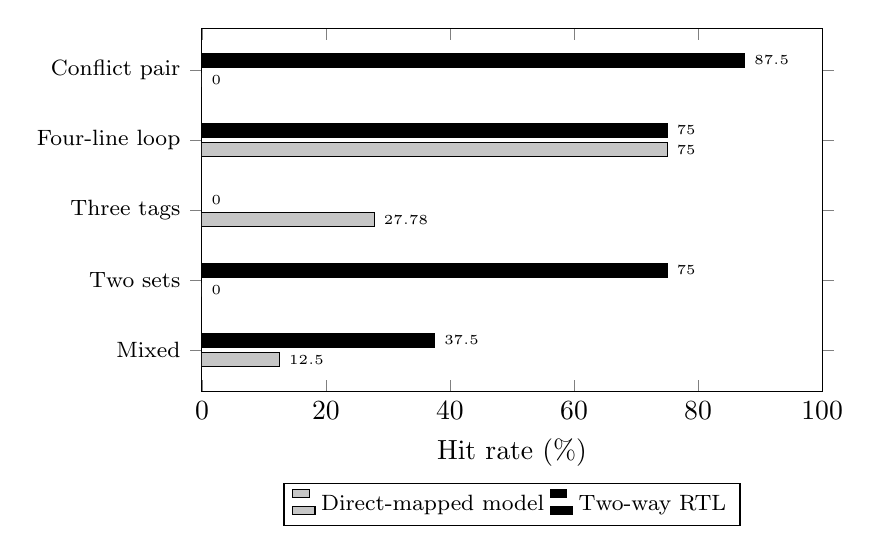
\begin{tikzpicture}
\begin{axis}[
  xbar, width=0.78\columnwidth, height=6.2cm,
  xmin=0, xmax=100, xlabel={Hit rate (\%)},
  symbolic y coords={Mixed,Two sets,Three tags,Four-line loop,Conflict pair},
  ytick=data, y tick label style={font=\footnotesize},
  bar width=5pt, nodes near coords, nodes near coords style={font=\tiny},
  legend style={at={(0.5,-0.25)}, anchor=north, legend columns=2, font=\footnotesize},
  enlarge y limits=0.15]
\addplot[fill=gray!45] coordinates {(0,Conflict pair) (75,Four-line loop) (27.78,Three tags) (0,Two sets) (12.5,Mixed)};
\addplot[fill=black] coordinates {(87.5,Conflict pair) (75,Four-line loop) (0,Three tags) (75,Two sets) (37.5,Mixed)};
\legend{Direct-mapped model, Two-way RTL}
\end{axis}
\end{tikzpicture}
\caption{Hit rates for selected traces, in percent. Direct-mapped values
are software-model results; two-way values are RTL simulation results.}
\label{fig:hits}
\end{figure}

The two-sets trace extends this effect to both sets: addresses 0 and 4
can coexist in one set while 1 and 5 coexist in the other. Four
compulsory misses are followed by twelve hits. Direct mapping suffers
repeated conflicts in both affected indices. The mixed trace shows a
smaller improvement because it combines useful reuse with further
replacements (Fig.~\ref{fig:hits}).

\subsection{When More Associativity Does Not Help}

Repeated access to one address produces the same result in both caches:
one compulsory miss and fifteen hits. The four-line loop also ties
because all four values fit without harmful conflicts in either
organization. A single traversal of sixteen unique addresses produces
no hits in either design. A one-byte cache line cannot make the next
sequential byte a hit merely by fetching the previous one.

The three-tags trace, $[0,2,4]$ repeated six times, is a counterexample
to a universal associativity benefit. All three addresses compete for
two ways in set~0. Under LRU, each access evicts the address needed
after the next access, so every reference misses. In the direct-mapped
model, address~2 occupies index~2 independently, while 0 and 4 compete
at index~0. Address~2 therefore hits on its final five appearances,
yielding $5/18 = 27.78\%$.

This outcome follows from the change in set partitioning at fixed
capacity. It does not indicate an LRU implementation error. A
replacement policy can only choose among the entries in the selected
set; it cannot borrow unused capacity from another set. Likewise, an
average across these hand-selected traces is not a general workload
performance estimate.

\subsection{Replacement Behavior at Individual Accesses}

\begin{table}[!t]
\caption{LRU Probe in Set 1}
\label{tab:lruprobe}
\centering
\begin{tabular}{cccc}
\toprule
Access & Outcome & Resident (way 0, way 1) & Next victim \\
\midrule
3 & Miss & 3, empty & Way 1 \\
5 & Miss & 3, 5 & Way 0 \\
3 & Hit  & 3, 5 & Way 1 \\
7 & Miss & 3, 7 & Way 0 \\
3 & Hit  & 3, 7 & Way 1 \\
5 & Miss & 3, 5 & Way 0 \\
3 & Hit  & 3, 5 & Way 1 \\
5 & Hit  & 3, 5 & Way 0 \\
\bottomrule
\end{tabular}
\end{table}

The resident-address pair in Table~\ref{tab:lruprobe} is ordered as
way~0, way~1. The fourth access replaces 5, and the sixth replaces 7,
while 3 survives because of its intervening hits. The expected hit/miss
sequence is M, M, H, M, H, M, H, H. RTL simulation produced four hits,
four backing-memory reads, and correct response data for every access.

The test also demonstrates why a fill must update LRU: after installing
a new byte, that byte represents the just-completed access. Leaving
replacement state unchanged could cause the newly filled entry to be
selected again even when the other way is older.

\subsection{Response Latency and Resource Analysis}

\begin{table}[!t]
\caption{Measured Two-Way Response Latency}
\label{tab:latency}
\centering
\begin{tabular}{lcc}
\toprule
Trace & Total elapsed cycles & Mean cycles/read \\
\midrule
Repeat & 19 & 1.1875 \\
Conflict pair & 22 & 1.3750 \\
Four-line loop & 28 & 1.7500 \\
One pass & 64 & 4.0000 \\
Three tags & 72 & 4.0000 \\
Two sets & 28 & 1.7500 \\
LRU probe & 20 & 2.5000 \\
Mixed & 46 & 2.8750 \\
\bottomrule
\end{tabular}
\end{table}

Table~\ref{tab:latency} sums acceptance-to-response latency for each
request. The totals agree with $H + 4M$ for every trace. This confirms
the intended hit bypass and miss-refill sequence under the integrated
memory model. It does not compare two hardware controllers, and it
should not be presented as an FPGA speedup against direct mapping.

The two-way cache array requires $4 \times (8 + 3 + 1) = 48$ logical
bits for data, tags, and validity. The two LRU bits bring the cache
storage total to 50 bits. An equal-capacity direct-mapped array requires
$4 \times (8 + 2 + 1) = 44$ bits. Thus, this configuration adds six
logical bits: four for wider tags and two for LRU. The comparison
excludes controller registers, memory-model state, and synthesized
logic.

The two-way datapath also includes two three-bit tag comparisons and a
data-way multiplexer, whereas the direct-mapped organization needs one
selected-tag comparison. Actual FPGA resource use depends on memory
inference, reset behavior, logic optimization, and the target device.
Logical bit counts are not LUT, flip-flop, or block-RAM counts.

\subsection{Limitations and Next Steps}

No FPGA device, constraints file, synthesis utilization, or post-route
timing report was available. The current array's asynchronous reads and
reset of all storage entries may affect RAM inference. These effects
must be checked with a chosen synthesis tool rather than assumed from
the Verilog declarations.

Further evaluation should implement a direct-mapped RTL baseline with
the same interface and memory latency, then synthesize both designs
under identical constraints. Useful additional tests include reset
during an outstanding miss, variable-latency memory, longer randomized
traces, and assertions for one response per accepted request.
Parameterization, multi-byte lines, and a documented write policy are
suitable architectural extensions.

% =====================================================================
\section{Individual Contributions}

The work was divided into five roles. Each member's commits are visible
in the repository history~\cite{repo}.

\textbf{Pranjal Shukla --- Architecture and Integration.} Finalized the
cache architecture and signal definitions, integrated all RTL modules
into the top-level \texttt{cache\_2way} module, and verified the
complete top-level cache. Ensured every member could explain the design.

\textbf{Ritesh Kumar --- Cache Storage and Address Decoder.} Implemented
the tag arrays, valid bits, data storage, and address decoding, and
tested both cache ways independently.

\textbf{Meghna Nair --- LRU Replacement Logic.} Implemented the LRU
bits, hit-based LRU updates, invalid-way selection, and victim
selection, and tested eviction behavior.

\textbf{Shreya Narayani --- Verification and Simulation.} Built the
Verilog testbenches, tested hit/miss conditions and LRU replacement,
captured waveform screenshots, and prepared the expected-versus-actual
results.

\textbf{Nikith Gowda B S --- Documentation and Repository.} Set up the
GitHub repository structure, created the IEEE report structure,
prepared the literature review and references, maintained the README
and architecture diagrams, and coordinated video editing and
submission.

% =====================================================================
\section{Conclusion}

The project realizes a four-line, read-only, two-way set-associative
cache with parallel lookup and exact one-bit-per-set LRU replacement.
Reproduced unit tests and the 53-check integration test support the
implemented decoding, selection, refill, and request-handshake behavior.
Eight supplementary traces matched an independent reference model and
returned the expected memory data.

The equal-capacity comparison demonstrates both the benefit and the
limit of flexible placement. An alternating conflict pair improves from
0\% to 87.50\% hits, while a three-address same-set loop favors direct
mapping. The defensible conclusion is that two-way LRU reduces
particular conflict patterns with modest logical-state overhead; a
general performance or FPGA-area claim requires a hardware baseline and
synthesis evidence.

% =====================================================================
\begin{thebibliography}{5}

\bibitem{repo}
Pranjal9005, ``2-Way-Set-Associative-Cache,'' GitHub repository, commit
c8b1374b16fa6555b47aa9e47d37a963e50767b8. Accessed: Nov. 16, 2026.
[Online]. Available:
\url{https://github.com/Pranjal9005/2-Way-Set-Associative-Cache}

\bibitem{cornell}
Cornell University, ``Caches,'' CS 3410, Spring 2025. Accessed: Nov. 16,
2026. [Online]. Available:
\url{https://www.cs.cornell.edu/courses/cs3410/2025sp/notes/caches.html}

\bibitem{berkeley}
University of California, Berkeley, ``Fully Associative Cache,'' CS 61C
Course Notes. Accessed: Nov. 16, 2026. [Online]. Available:
\url{https://notes.cs61c.org/content/caches-ii/fully-associative/}

\bibitem{jouppi}
N. P. Jouppi, ``Improving direct-mapped cache performance by the
addition of a small fully-associative cache and prefetch buffers,'' in
\emph{Proc. 17th Annu. Int. Symp. Computer Architecture}, 1990,
pp. 364--373, doi: 10.1145/325164.325162.

\bibitem{icarus}
Icarus Verilog, ``Getting Started With Icarus Verilog.'' Accessed:
Nov. 16, 2026. [Online]. Available:
\url{https://steveicarus.github.io/iverilog/usage/getting_started.html}

\end{thebibliography}

\end{document}
